\documentclass{beamer}
\beamertemplatenavigationsymbolsempty
\usepackage{amsmath, amssymb, hyperref, graphics}
\usepackage{tikz}

\title{Graph Theory Lecture 14}

\begin{document}
\begin{frame}{Euler's Theorem: What's wrong with this picture?}
            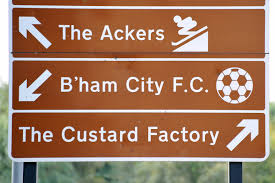
\includegraphics[width=\textwidth]{Pictures/footballsign.jpeg}
\end{frame}

\begin{frame}{Theorem: Every football has 12 pentagons}
  We will prove this theorem today as a corollary to Euler's Theorem.

  \begin{definition} Suppose that a graph $G$ is drawn on the sphere $S^2$ so that no edges cross.  Then $G$ cuts the sphere into a finite number of pieces called the \emph{faces} of $G$.
  \end{definition}

  \begin{block}{Intuition / origin of name:}
    Think about the cube (or more generally a polyhedron).
    \begin{description}
    \item[Vertices] Corners
      \item[Edges] Where two cube faces meet
       \item[Faces] Faces of cube
      \end{description}

    \end{block}
 
\end{frame}

\begin{frame}{Counting vertices, faces and edges}
  $$\begin{array}{c|c|c|c}
    \text{Graph} & V & E & F  \\ \hline
    C_n & n & n & 2 \\
    W_n & n+1 & 2n & n+1 \\
    K_4=\text{Tetrahedra} & 4 & 6 & 4 \\
    \text{Cube} & 8 & 12 & 6 \\
    \text{Octahedron} & 6 & 12 & 8 \\
    \text{Dodecahedron} & 20 & 30 & 12 \\
    \text{Icosahedron} & 12 & 30 & 20 \\
    \text{Make your own} & & & 
  \end{array}
  $$
\begin{block}{What patterns do you see?}
  \end{block}
  \end{frame}

\begin{frame}{Euler's Formula}
  \begin{theorem}{Euler's formula for graphs on the sphere}
    Let $G$ be a graph drawn on the sphere without edges crossing.  Let $V$ and $E$ be the number of edges and vertices of $G$, respectively, and let $F$ be the number of faces of the drawing.  Then
    $$V-E+F=2$$
    \end{theorem}

  \begin{block}{Cultural remarks}
    \begin{itemize}
    \item Euler stated for polytopes, didn't prove rigorously
    \item Imre Lakatos's \emph{Proof and Refutations} important work in philosophy of math tracing this theorem
    \item Beginings of topology: $V-E+F$ is called the \emph{Euler characteristic}
      \end{itemize}
    \end{block}

  
  \end{frame}
\begin{frame}{How to use Euler's Theorem}
  \begin{block}{One shortcoming:}
    Only one equation, but three variables: $V,E,F$
    \end{block}

  \begin{block}{Handshaking can give us another relation:}
    On a football, every vertex has degree three.
    $$2E=\sum_{v\in V(G)} d(w)=\sum_{v\in V(G)} 3=3V$$
  \end{block}

  \begin{block}{Similar handshaking between faces and edges}

    Let the \emph{degree} $d(f)$ of a face $f$ be the number of edges around it.
    \begin{itemize}
\item    Then each edge meets two faces 
\item    Each face $f$ meets $d(f)$ edges 
    \end{itemize}
    $$\sum_{f \text{ face}} d(f)=2E$$
\end{block}
    
  

  \end{frame}

\begin{frame}{Proof that a football has 12 pentagons}
\begin{definition}
  A \emph{football}, we mean a graph $G$ drawn on the plane where:
  \begin{itemize}
  \item Every vertex $v\in G$ has degree 3
  \item Every face $f$ has degree 5 or 6
  \end{itemize}
\end{definition}

  Suppose there are $P$ pentagons and $H$ hexagons, so $F=P+H$.

\begin{block}{Basic recipe for applying Euler's theorem:}
Combine the following ingredients and stir well:
  \begin{itemize}
\item  Euler's Theorem: $V-E+P+H=2$
\item Vertex-edge Handshaking: $3V=2E$
\item Face-edge Handshaking: $5P+6H=2E$
  \end{itemize}
\end{block}


  

\end{frame}
  
\end{document}
